\documentclass[border = 5mm]{standalone}

\usepackage{tikz}
\usepackage{upquote}
\usetikzlibrary{calc, intersections}
% upquote = straight quotes to get for instance A'
% calc - extend lines beyond their end points
% intersections - to get points of intersection of the lines

\begin{document}
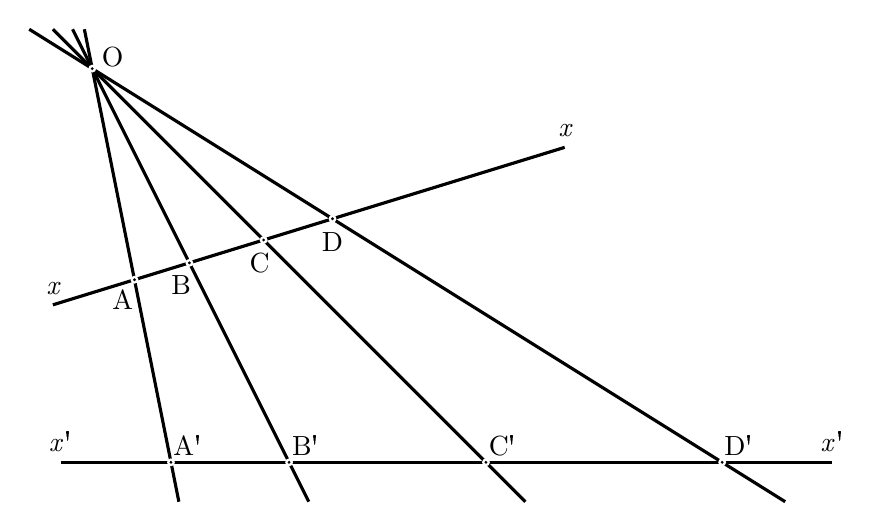
\begin{tikzpicture}[line width=0.4mm]

% Initial coordinates for O and A', B', C', D'
\coordinate (O) at (0,5);

\coordinate (A') at (1,0);
\coordinate (B') at (2.5,0);
\coordinate (C') at (5,0);
\coordinate (D') at (8,0);

% Label these points
\node at ([shift=({30:.3})]O) {O};

\foreach \i\j in {A'/A, B'/B, C'/C, D'/D} {
\node at ([shift=({45:.3})]\i) {\j\textquotesingle};
}

% Draw line x', i.e., A'D' but extended beyond the points
\draw ($(A')!-0.2!(D')$) node[above] {\itshape{x}\textnormal{\textquotesingle}} -- ($(A')!1.2!(D')$) node[above] {\itshape{x}\textnormal{\textquotesingle}};

% Draw lines from O to line x' extended.
% They have names (a, b, c, d). Those names allow intersections to be found.
% The names are not labels for the lines that appear in the figure,
% but the lines could have such labels (see Figure 4.2)
\foreach \i\j in {a/A', b/B', c/C', d/D'} {
  \draw [name path global=\i] ($(O)!-0.1!(\j)$) -- ($(O)!1.1!(\j)$);
}

% Draw line x , i.e., AD
\coordinate (X) at (-.5,2);
\coordinate (Y) at (6,4);
\draw [name path global=x] (X) node[above] {\itshape{x}} -- (Y) node[above] {\itshape{x}};

% Intersections of x with a, b, c, d
%\foreach \i\j in {a/A, b/B, c/C, d/D} {
%\path [name intersections={of=\i and x, by=\j];
%}

\path [name intersections={of=a and x, by=A}];
\path [name intersections={of=b and x, by=B}];
\path [name intersections={of=c and x, by=C}];
\path [name intersections={of=d and x, by=D}];

\foreach \i\j in {A/240, B/250, C/260, D/270} {
  \node at ([shift=({\j:.3})]\i) {\i};
}

%\node at ([shift=({240:.3})]A) {A};
%\node at ([shift=({250:.3})]B) {B};
%\node at ([shift=({260:.3})]C) {C};
%\node at ([shift=({270:.3})]D) {D};

% Draw the points
\foreach \x in {A, ..., D, A', B', C', D', O} {
  \fill[white] (\x) circle(0.05);
  \fill[black] (\x) circle(0.02); 
}


\end{tikzpicture}
\end{document}
